\documentclass[10pt]{article}

\usepackage[utf8]{inputenc}
\usepackage{latexsym,amsfonts,amssymb,amsthm,amsmath}
\setlength{\parindent}{0in}
\setlength{\parskip}{\baselineskip}
\setlength{\oddsidemargin}{0in}
\setlength{\textwidth}{6.5in}
\setlength{\textheight}{8.8in}
\setlength{\topmargin}{0in}
\setlength{\headheight}{18pt}

\usepackage[a4paper,margin=1in,footskip=0.25in]{geometry}

\usepackage{listings}
\usepackage{color} %red, green, blue, yellow, cyan, magenta, black, white
\definecolor{mygreen}{RGB}{28,172,0} % color values Red, Green, Blue
\definecolor{mylilas}{RGB}{170,55,241}

\usepackage{graphicx}
\graphicspath{{../output/}}

\def\code#1{\texttt{#1}} % Monospacing shortcut: Use \code{}

\usepackage[colorlinks=true, urlcolor=blue, linkcolor=blue]{hyperref}

\usepackage{verbatim} % For including raw text files in the pdf
\usepackage{float} % For keeping figures in the section where they were called 

\title{PHYS 410 Project 2}
\author{Gavin Pringle, 56401938}

%%%%%%%%%%%%%%%%%%%%%%%%%%%%%%%%%%%%%%%%%%%%%%%%%%%%%%%%%%%%%%%%%%%%%%%%%%%%%%%%%%%%%%%%%%%%%%%%%%%%%%%
% Start of document
%%%%%%%%%%%%%%%%%%%%%%%%%%%%%%%%%%%%%%%%%%%%%%%%%%%%%%%%%%%%%%%%%%%%%%%%%%%%%%%%%%%%%%%%%%%%%%%%%%%%%%%
\begin{document}

\maketitle

\lstset{language=Matlab,%
    %basicstyle=\color{red},
    breaklines=true,%
    morekeywords={matlab2tikz},
    keywordstyle=\color{blue},%
    morekeywords=[2]{1}, keywordstyle=[2]{\color{black}},
    identifierstyle=\color{black},%
    stringstyle=\color{mylilas},
    commentstyle=\color{mygreen},%
    showstringspaces=false,%without this there will be a symbol in the places where there is a space
    numbers=left,%
    numberstyle={\tiny \color{black}},% size of the numbers
    numbersep=9pt, % this defines how far the numbers are from the text
    emph=[1]{for,end,break},emphstyle=[1]\color{red}, %some words to emphasise
    %emph=[2]{word1,word2}, emphstyle=[2]{style},
    literate=%
        {ö}{{\"o}}1 % Maps ö to its LaTeX representation
        {Ψ}{{$\Psi$}}1 % Maps Ψ to its LaTeX representation 
        {ψ}{{$\psi$}}1 % Maps ψ to its LaTeX representation       
}

%%%%%%%%%%%%%%%%%%%%%%%%%%%%%%%%%%%%%%%%%%%%%%%%%%%%%%%%%%%%%%%%%%%%%%%%%%%%%%%%%%%%%%%%%%%%%%%%%%%%%%%
% Introduction
%%%%%%%%%%%%%%%%%%%%%%%%%%%%%%%%%%%%%%%%%%%%%%%%%%%%%%%%%%%%%%%%%%%%%%%%%%%%%%%%%%%%%%%%%%%%%%%%%%%%%%%
\subsection*{Introduction}

In this project, the time-dependent Schrödinger equation is solved numerically in both one dimension
and two dimensions. In both cases, solutions account for a time-independent potential term $V$, which
takes the form of a rectangular barrier or well, a double slit (in 2d only), or is zero everywhere. 
The MATLAB script \code{sch\_1d\_cn.m} implements the Crank-Nicolson discretization approach to solve 
the Schrödinger equation in 1d, while the script \code{sch\_2d\_adi.m} implements the 
alternating-direction-implicit (ADI) method to solve the equation in 2d. 

The 1d case is tested by conducting convergence testing in the file \code{ctest\_1d.m} which checks 
for solution convergence among increasing discretization levels. A similar convergence test is done 
for two dimensions in the file \code{ctest\_2d.m}. For the 1d case, the solution "excess fractional
probability" is also examined in the files \code{barrier\_survey.m} and \code{well\_survey.m}, which
provides insights into how much time the quantum particle is spending in a certain location. Lastly,
videos of the 2d wave function scattering off a rectangular barrier or well, and producing 
self-interference through a double slit are created using the scripts \code{video\_rec\_bar.m},
\code{video\_rec\_well.m}, and \code{video\_double\_slit.m}.

%%%%%%%%%%%%%%%%%%%%%%%%%%%%%%%%%%%%%%%%%%%%%%%%%%%%%%%%%%%%%%%%%%%%%%%%%%%%%%%%%%%%%%%%%%%%%%%%%%%%%%%
% Review of Theory
%%%%%%%%%%%%%%%%%%%%%%%%%%%%%%%%%%%%%%%%%%%%%%%%%%%%%%%%%%%%%%%%%%%%%%%%%%%%%%%%%%%%%%%%%%%%%%%%%%%%%%%
\subsection*{Review of Theory}

\subsubsection*{1d Schrödinger Equation}

The 1d Schrödinger Equation PDE is given by the following equation:
\begin{equation}\label{sch_1d}
i\psi(x,t)_t = -\psi_{xx} + V(x,t)\psi
\end{equation}
where the wave function, $\psi(x,t)$, is complex. The equation is to be solved on the domain
$$0\leq x \leq 1, \quad 0 \leq t \leq t_{\textrm{max}}$$
subject to initial and boundary conditions
\begin{equation}\label{sch_1d_IC}
\psi(x,0) = \psi_0(x)
\end{equation}
\begin{equation}\label{sch_1d_BC}
\psi(0,t) = \psi(1,t) = 0
\end{equation}

The family of exact solutions to (\ref{sch_1d}) is
\begin{equation}\label{1d_exact_soln}
\psi(x,t) = e^{-i m^2 \pi^2 t} \sin(m \pi x)
\end{equation}
where m is a positive integer. 

Since the modulus squared of the wave function represents the probability density, 
$\rho = |\psi|^2 = \psi \psi^*$, the "running integral" of the probability density represents
the probability that the particle is to the left of $x$ at any given time $t$:
\begin{equation}\label{prob_den}
P(x,t) = \int_0^x \psi(\tilde{x}, t) \psi^*(\tilde{x}, t) d\tilde{x}
\end{equation}
Note that equation (\ref{prob_den}) only computes the correct probability if the wave function 
is properly normalized such that $P(1,t) = 1$. Even if it is not so normalized, we should have
$$P(1,t) = \textrm{conserved to level of solution error}$$

\subsubsection*{2d Schrödinger Equation}

The 2d Schrödinger Equation PDE is given by the following equation:
\begin{equation}\label{sch_2d}
\psi_t = i(\psi_{xx} + \psi_{yy}) - iV(x,y)\psi
\end{equation}
where the wave function, $\psi(x,y,t)$, is complex. The equation is to be solved on the domain
$$0\leq x \leq 1, \quad 0 \leq y \leq 1, \quad 0\leq t \leq t_{\textrm{max}}$$
subject to initial and boundary conditions
\begin{equation}\label{sch_2d_IC}
\psi(x,y,0) = \psi_0(x,y)
\end{equation}
\begin{equation}\label{sch_2_BC}
\psi(0,y,t) = \psi(1,y,t) = \psi(x,0,t) = \psi(x,1,t) = 0
\end{equation}

A family of exact solutions to (\ref{sch_2d}) is given by
\begin{equation}\label{2d_exact_soln}
\psi(x,y,t) = e^{-i (m_x^2 + m_y^2) \pi^2 t} \sin(m_x \pi x) \sin(m_y \pi y)
\end{equation}

%%%%%%%%%%%%%%%%%%%%%%%%%%%%%%%%%%%%%%%%%%%%%%%%%%%%%%%%%%%%%%%%%%%%%%%%%%%%%%%%%%%%%%%%%%%%%%%%%%%%%%%
% Numerical approach
%%%%%%%%%%%%%%%%%%%%%%%%%%%%%%%%%%%%%%%%%%%%%%%%%%%%%%%%%%%%%%%%%%%%%%%%%%%%%%%%%%%%%%%%%%%%%%%%%%%%%%%
\subsection*{Numerical Approach}

\subsubsection*{1d Schrödinger Equation}

We discretize the domain by introducing the discretization level $l$, and the ratio of temporal to 
mesh spacings $\lambda$. The script \code{sch\_1d\_cn.m} takes $t_{\textrm{max}}$, $l$, and $\lambda$ 
as parameters.
$$\lambda = \frac{\Delta t}{\Delta x}$$
$$n_x = 2^l + 1$$
$$\Delta x = 2^{-l}$$
$$\Delta t = \lambda \Delta x$$
$$n_t = \textrm{round} (t_{\textrm{max}} / \Delta t) + 1$$

When the Crank-Nicolson discretization approach is applied to equations (\ref{sch_1d}) - 
(\ref{sch_1d_BC}), the following relation is reached:  
\begin{align}\label{CN}
i \frac{\psi_j^{n+1} - \psi_j^n}{\Delta t} = \frac{1}{2} \left( 
\frac{\psi_{j+1}^{n+1} - 2\psi_j^{n+1} + \psi_{j-1}^{n+1}}{\Delta x^2} 
+ \frac{\psi_{j+1}^n - 2\psi_j^n + \psi_{j-1}^n}{\Delta x^2} \right)
&+ \frac{1}{2} V_j^{n+\frac{1}{2}} \left(\psi_j^{n+1} + \psi_j^n \right) \nonumber \\
j = 2, 3, \dots, n_x - 1, \, n = 1, 2, \dots, n_t &- 1
\end{align}
which is subject to the initial and boundary conditions:
$$\psi_1^{n+1} = \psi_{n_x}^{n+1} = 0, \quad n = 1, 2, \dots, n_t - 1$$
$$\psi_j^1 = \psi_0(x_j), \quad j = 1, 2, \dots, n_x$$

If (\ref{CN}) is rearranged such that each term contains a singular $\psi$ term, we reach equation
(\ref{CN_rearranged}). This is the equation that defines the tridiagonal system used for solving the 
1d Schrödinger equation. The method for implementing this equation in code is described later in the 
implementation section.
\begin{align}\label{CN_rearranged}
\frac{1}{2 \Delta x^2}\psi_{j+1}^{n+1} + & \left( \frac{i}{\Delta t} - \frac{1}{\Delta x^2}
-\frac{1}{2}V_j \right) \psi_j^{n+1} + \frac{1}{2 \Delta x^2} \psi_{j-1}^{n+1} \nonumber \\
& = -\frac{1}{2 \Delta x^2} \psi_{j+1}^n + \left(\frac{i}{\Delta t} + \frac{1}{\Delta x^2}
+ \frac{1}{2}V_j \right) \psi_j^n - \frac{1}{2 \Delta x^2} \psi_{j-1}^n
\end{align}

The script \code{sch\_1d\_cn.m} additionally takes parameters \code{idtype}, \code{idpar}, 
\code{vtype}, and \code{vpar}. \code{idtype} and \code{idpar} define the initial conditions, 
which takes the form of an exact family for \code{idtype == 0}:
$$\psi(x,0) = \sin(m \pi x)$$
or of a boosted Gaussian for \code{idtype == 1}: 
$$\psi(x,0) = e^{i p x} e^{-((x - x_0)/\delta)^2}$$
\code{vtype} and \code{vpar} define the time-independent potential which takes the form of no 
potential for \code{vtype == 0}:
$$V(x) = 0$$
or of a rectangular barrier or well for \code{vtype == 1}:
$$V(x) =
\begin{cases} 
0 & \text{for } x < x_{\text{min}}, \\
V_c & \text{for } x_{\text{min}} \leq x \leq x_{\text{max}}, \\
0 & \text{for } x > x_{\text{max}}.
\end{cases} $$

\subsubsection*{2d Schrödinger Equation}

For the 2d case, the domain is discretized in a similar way by introducing the discretization 
level $l$ and the ratio of temporal to mesh spacings $\lambda$. In the 2d scenario, we always 
assume $x$ and $y$ steps are equal. The script \code{sch\_2d\_adi.m} takes $t_{\textrm{max}}$, $l$, 
and $\lambda$ as parameters.
$$\lambda = \frac{\Delta t}{\Delta x} = \frac{\Delta t}{\Delta y}$$
$$n_x = n_y = 2^l + 1$$
$$\Delta x = \Delta y = 2^{-l}$$
$$\Delta t = \lambda \Delta x$$
$$n_t = \textrm{round}(t_{\textrm{max}} / \Delta t) + 1$$

When ADI discretization method is applied to equation (\ref{sch_2d}), the following relations are 
reached:
\begin{align}\label{ADI_1}
\left( 1 - i \frac{\Delta t}{2} \partial_{xx}^h \right) \psi_{i,j}^{n+\frac{1}{2}} &=
\left( 1 + i \frac{\Delta t}{2} \partial_{xx}^h \right)
\left( 1 + i \frac{\Delta t}{2} \partial_{yy}^h - i \frac{\Delta t}{2} V_{i,j} \right) \psi_{i,j}^n,
\nonumber \\ i &= 2,3,\ldots,n_x-1, \quad j = 2,3,\ldots,n_y-1, \quad n = 1,2,\ldots,n_t-1.
\end{align}
\begin{align}\label{ADI_2}
\left( 1 - i \frac{\Delta t}{2} \partial_{yy}^h + i \frac{\Delta t}{2} V_{i,j} \right) 
\psi_{i,j}^{n+1} &= \psi_{i,j}^{n+\frac{1}{2}},
\nonumber \\ i = 2,3,\ldots,n_x-1, \quad j &= 2,3,\ldots,n_y-1, \quad n = 1,2,\ldots,n_t-1.
\end{align}
Where it is understood that $\psi^{n+1}$ is found by first solving for $\psi^{n+\frac{1}{2}}$ via 
equation (\ref{ADI_1}). Both (\ref{ADI_1}) and (\ref{ADI_2}) are subject to the initial and 
boundary conditions:
$$\psi_{i,j}^1 = \psi_0 (x_i, y_j)$$
$$\psi_{1,j}^n = \psi_{n_x,j}^n = \psi_{i,1}^n = \psi_{i,n_y}^n = 0$$
The operators $\partial_{xx}^h$ and $\partial_{yy}^h$ are defined as:
$$\partial_{xx}^h u_{i,j}^n \equiv \frac{u_{i+1,j}^n - 2u_{i,j}^n + u_{i-1,j}^n}{\Delta x^2}$$
$$\partial_{yy}^h u_{i,j}^n \equiv \frac{u_{i,j+1}^n - 2u_{i,j}^n + u_{i,j-1}^n}{\Delta y^2}$$

The left-hand-side of equation (\ref{ADI_1}) can be rearranged into the following form for 
computing the sparse matrix for the first tridiagonal system:
\begin{equation}\label{n_half_LHS}
-\frac{i \Delta t}{2 \Delta x^2} \psi_{i+1,j}^{n+\frac{1}{2}} + \left(1 + 
\frac{i \Delta t}{\Delta x^2} \right) \psi_{i,j}^{n+\frac{1}{2}} - \frac{i \Delta t}{2 \Delta x^2} 
\psi_{i-1,j}^{n+\frac{1}{2}}
\end{equation}
The right-hand-side of equation (\ref{ADI_1}) is not expanded due to its complexity, but is instead
reduced to two steps of computation. Equation (\ref{n_half_RHS_1}) shows the action of the rightmost
parenthesis on $\psi_{i,j}^n$ in equation (\ref{ADI_1}). The output of this action is labelled as 
$f^*$.
\begin{equation}\label{n_half_RHS_1}
\frac{i \Delta t}{2 \Delta y^2} \psi_{i,j+1}^{n} + \left(1 - i \Delta t \left(\frac{1}{\Delta y^2}
+ \frac{V_{i,j}}{2} \right) \right) \psi_{i,j}^n + \frac{i \Delta t}{2 \Delta y^2} \psi_{i,j-1}^n
= f^*
\end{equation}
The action of the second from right parenthesis in equation (\ref{ADI_1}) on $f^*$ is then
shown in equation (\ref{n_half_RHS_2}).
\begin{equation}\label{n_half_RHS_2}
\frac{i \Delta t}{2 \Delta x^2} f_{i+1}^* + \left(1 - \frac{i \Delta t}{\Delta x^2} \right) f_i^*
+ \frac{i \Delta t}{2 \Delta x^2} f_{i-1}^* = f
\end{equation}
Equations (\ref{n_half_LHS}), (\ref{n_half_RHS_1}) and (\ref{n_half_RHS_2}) define the first
tridiagonal system in the ADI scheme, for which the implementation in code is described later in the 
implementation section. 

The output of the above tridiagonal system is then fed into the second tridiagonal system in the ADI 
scheme, which comes from rearranging equation (\ref{ADI_2}):
\begin{equation}\label{n_full}
-\frac{i \Delta t}{2 \Delta y^2} \psi_{i,j+1}^{n+1} + \left(1 + \frac{i \Delta t}{\Delta y^2} + 
\frac{i \Delta t}{2} V_{i,j} \right) \psi_{i,j}^{n+1} - \frac{i \Delta t}{2 \Delta y^2} 
\psi_{i,j-1}^{n+1} = \psi_{i,j-1}^{n+\frac{1}{2}}
\end{equation}
How equations (\ref{n_half_LHS}), (\ref{n_half_RHS_1}), (\ref{n_half_RHS_2}), and (\ref{n_full})
are implemented in code is described in detail in the implementation section of this report. 

The script \code{sch\_2d\_adi.m} additionally takes parameters \code{idtype}, \code{idpar}, 
\code{vtype}, and \code{vpar}. \code{idtype} and \code{idpar} define the initial conditions, 
which takes the form of an exact family for \code{idtype == 0}:
$$\psi(x,y,0) = \sin(m_x \pi x) \sin(m_y \pi y)$$
or of a boosted Gaussian for \code{idtype == 1}: 
$$\psi(x,y,0) = e^{i p_x x} e^{i p_y y} e^{-((x - x_0)^2 / \delta_x^2 + (y - y_0)^2 / \delta_y^2)}$$
\code{vtype} and \code{vpar} define the time-independent potential which takes the form of no 
potential for \code{vtype == 0}:
$$V(x,y) = 0$$
or of a rectangular barrier or well for \code{vtype == 1}:
$$V(x, y) = 
\begin{cases} 
V_c & \text{for } (x_{\min} \leq x \leq x_{\max}) \text{ and } (y_{\min} \leq y \leq y_{\max}) \\
0 & \text{otherwise}
\end{cases}$$
or of a double slit potential for \code{vtype == 2}:
$$j' = (n_y - 1) / 4 + 1$$
$$V_{i,j'} = V_{i,j'+1} = 0 \quad \text{for} \quad 
\left[ (x_1 \leq x_i) \ \text{and} \ (x_i \leq x_2) \right] \ \text{or} \ 
\left[ (x_3 \leq x_i) \ \text{and} \ (x_i \leq x_4) \right]$$
$$V_{i,j'} = V_{i,j'+1} = V_c \quad \text{otherwise}$$
$$V_{i,j} = 0 \quad \text{for} \quad j \neq (j' \ \text{or} \ j'+1)$$

%%%%%%%%%%%%%%%%%%%%%%%%%%%%%%%%%%%%%%%%%%%%%%%%%%%%%%%%%%%%%%%%%%%%%%%%%%%%%%%%%%%%%%%%%%%%%%%%%%%%%%%
% Implementation
%%%%%%%%%%%%%%%%%%%%%%%%%%%%%%%%%%%%%%%%%%%%%%%%%%%%%%%%%%%%%%%%%%%%%%%%%%%%%%%%%%%%%%%%%%%%%%%%%%%%%%%
\subsection*{Implementation}

\subsubsection*{1d Tridiagonal System}

% Reference sch_1d_cn  

\subsubsection*{2d Tridiagonal System}

% Reference sch_2d_adi

%%%%%%%%%%%%%%%%%%%%%%%%%%%%%%%%%%%%%%%%%%%%%%%%%%%%%%%%%%%%%%%%%%%%%%%%%%%%%%%%%%%%%%%%%%%%%%%%%%%%%%%
% Results
%%%%%%%%%%%%%%%%%%%%%%%%%%%%%%%%%%%%%%%%%%%%%%%%%%%%%%%%%%%%%%%%%%%%%%%%%%%%%%%%%%%%%%%%%%%%%%%%%%%%%%%
\subsection*{Results}

\subsubsection*{1d Schrödinger Equation}

% Describe convergence test (don't need to explain from scratch) and show results

\begin{figure}[H]
\centering
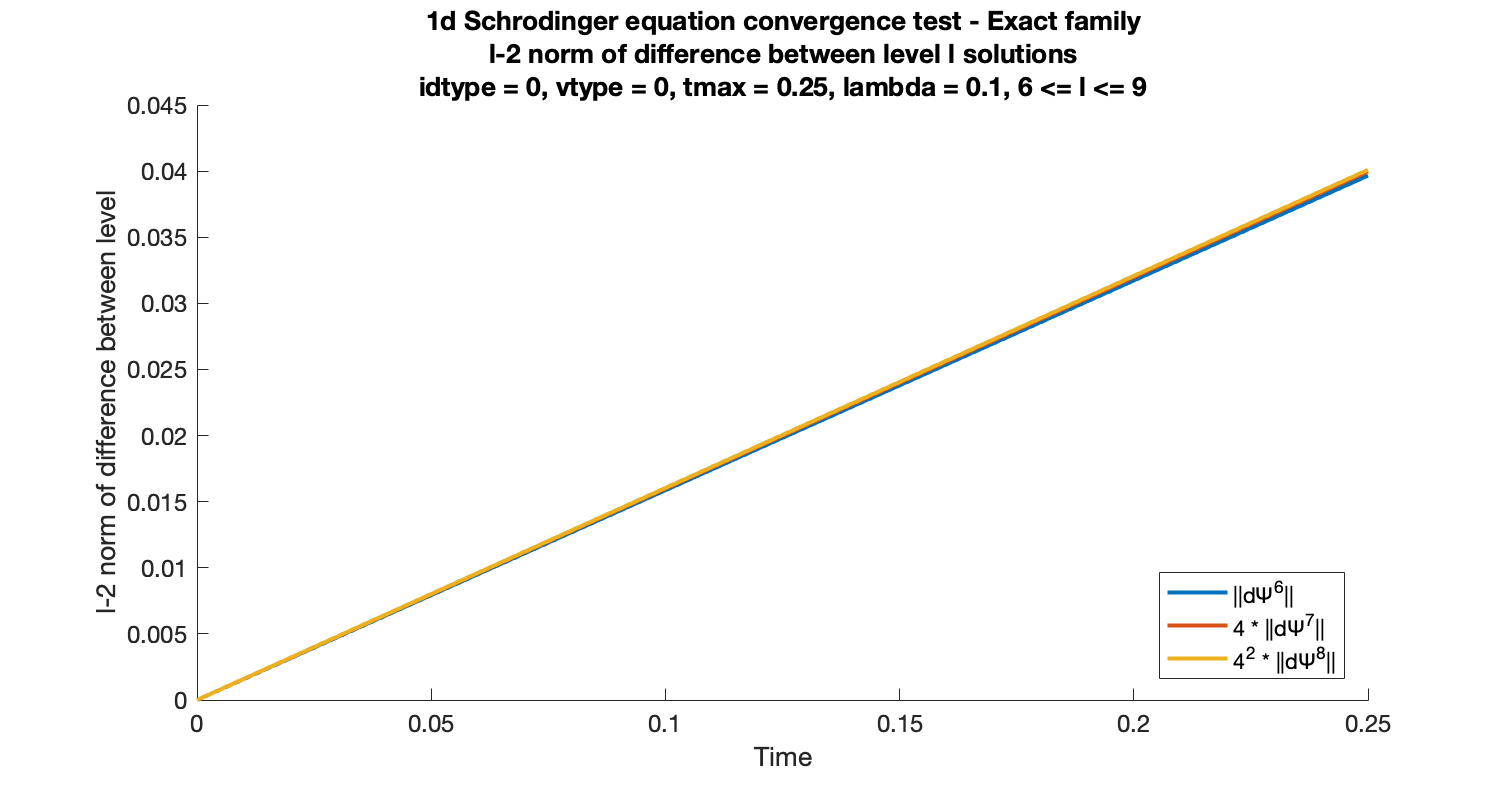
\includegraphics[width=0.95\textwidth]{problem1/ctest_1d-1.png}
\caption{Output 1 of \code{ctest\_1d.m} - 
l-2 norm of difference between discretization level solutions for exact family initial conditions.}
\end{figure}

\begin{figure}[H]
\centering
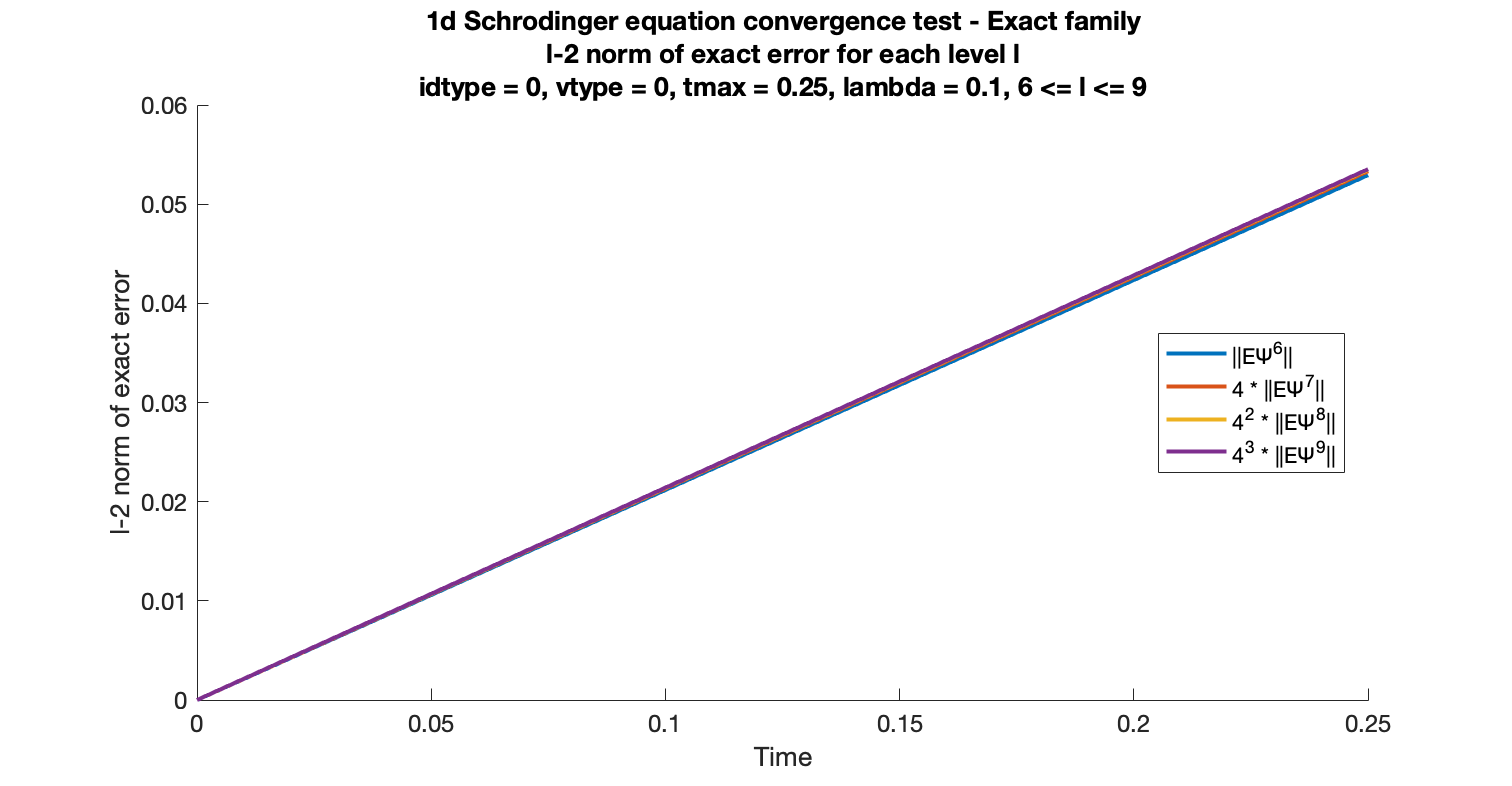
\includegraphics[width=0.95\textwidth]{problem1/ctest_1d-2.png}
\caption{Output 2 of \code{ctest\_1d.m} - 
l-2 norm of exact error at each discretization level for exact family initial conditions.}
\end{figure}

\begin{figure}[H]
\centering
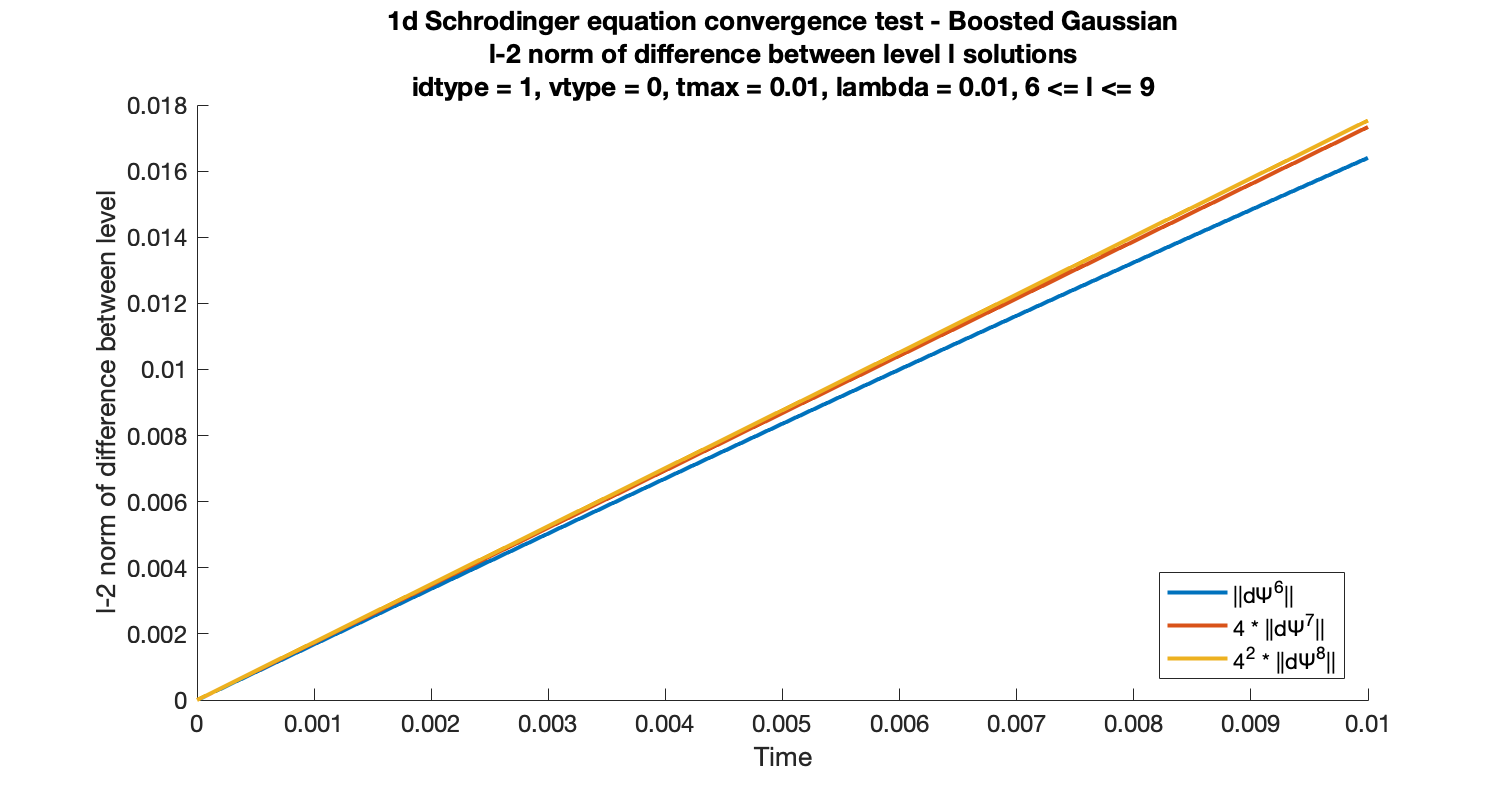
\includegraphics[width=0.95\textwidth]{problem1/ctest_1d-3.png}
\caption{Output 3 of \code{ctest\_1d.m} - 
l-2 norm of difference between discretization level solutions for boosted Gaussian initial 
conditions.}
\end{figure}

% Describe surveys (explain what lnFe is) and show results 

\begin{figure}[H]
\centering
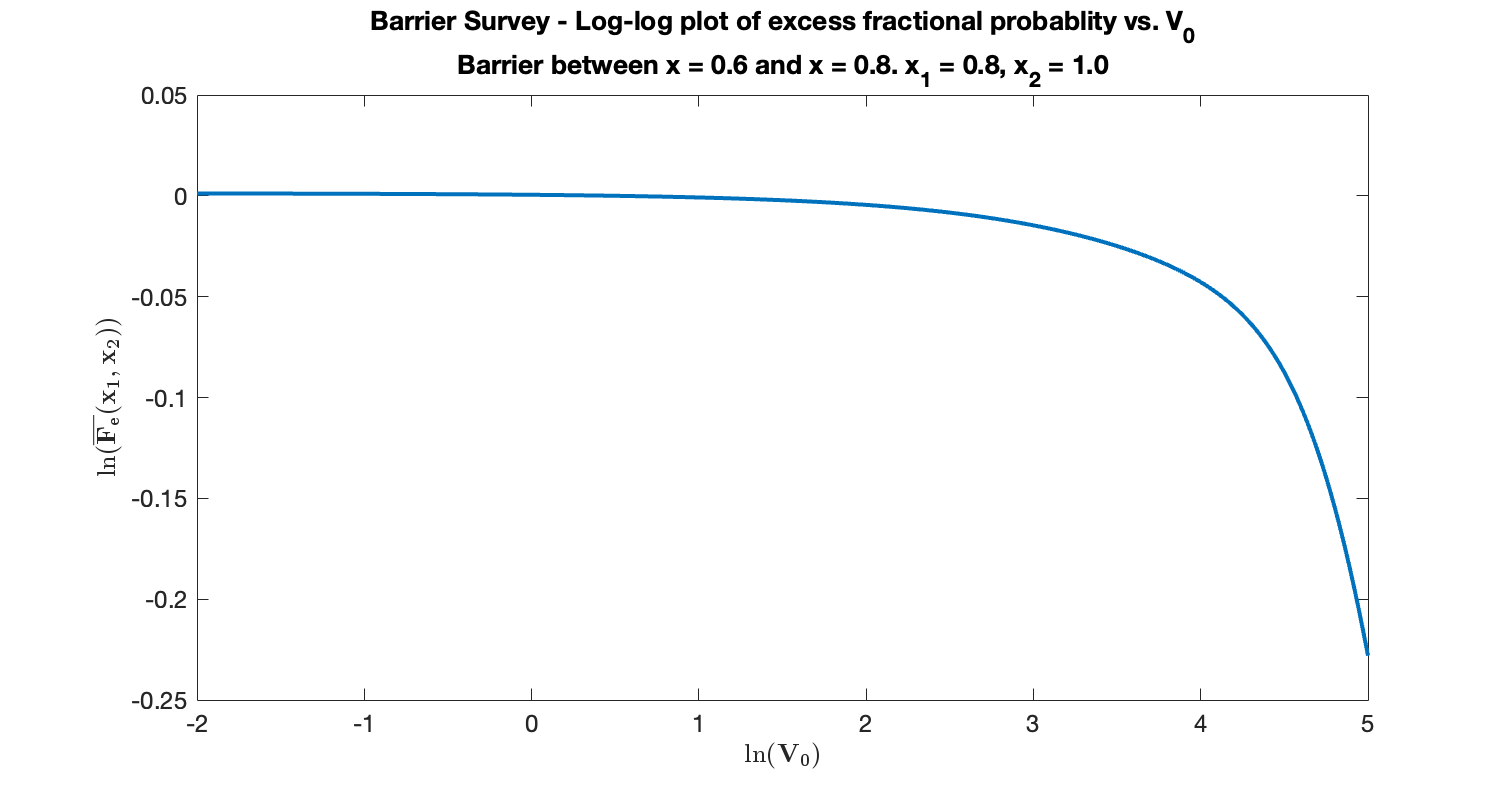
\includegraphics[width=0.95\textwidth]{problem1/barrier_1d.png}
\caption{Output of \code{barrier\_1d.m} - 
Log-log plot of excess fractional probability vs. $V_0$ for 1d potential barrier.}
\end{figure}

\begin{figure}[H]
\centering
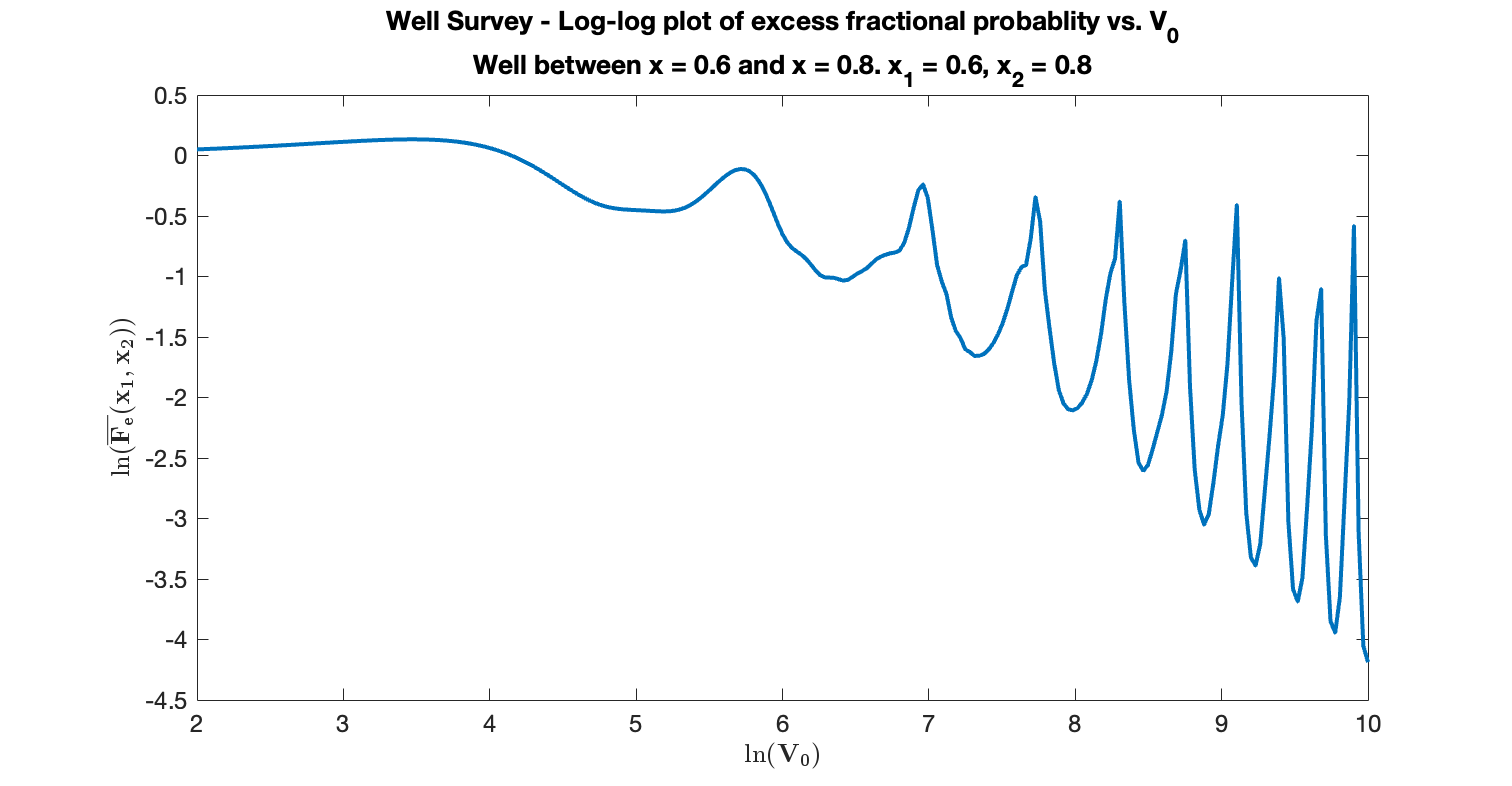
\includegraphics[width=0.95\textwidth]{problem1/well_1d.png}
\caption{Output of \code{well\_1d.m} - 
Log-log plot of excess fractional probability vs. $V_0$ for 1d potential well.}
\end{figure}

\subsubsection*{2d Schrödinger Equation}

% Describe convergence test (don't need to explain from scratch) and show results

\begin{figure}[H]
\centering
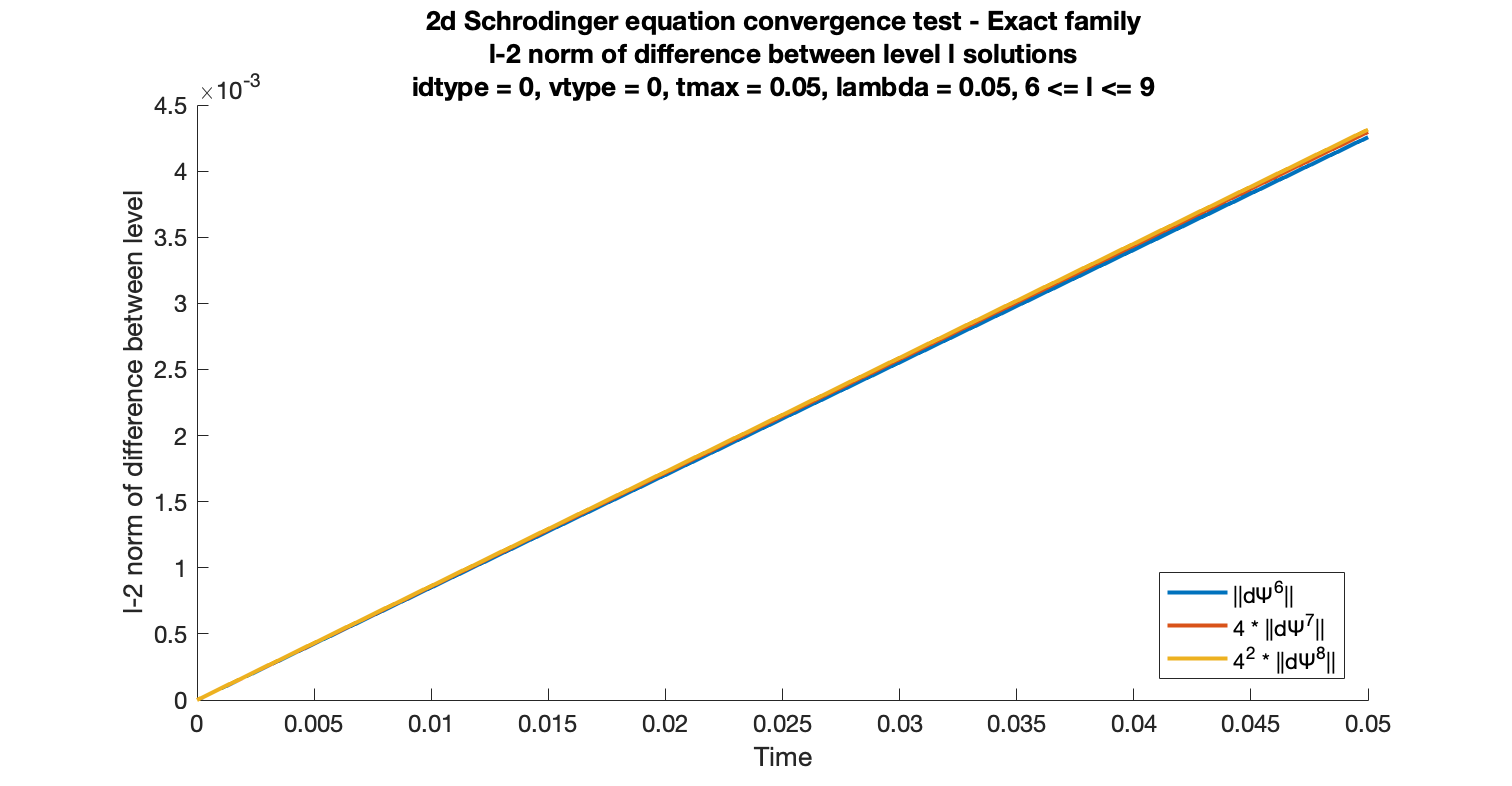
\includegraphics[width=0.95\textwidth]{problem2/ctest_2d-1.png}
\caption{Output 1 of \code{ctest\_2d.m} - 
l-2 norm of difference between discretization level solutions.}
\end{figure}

\begin{figure}[H]
\centering
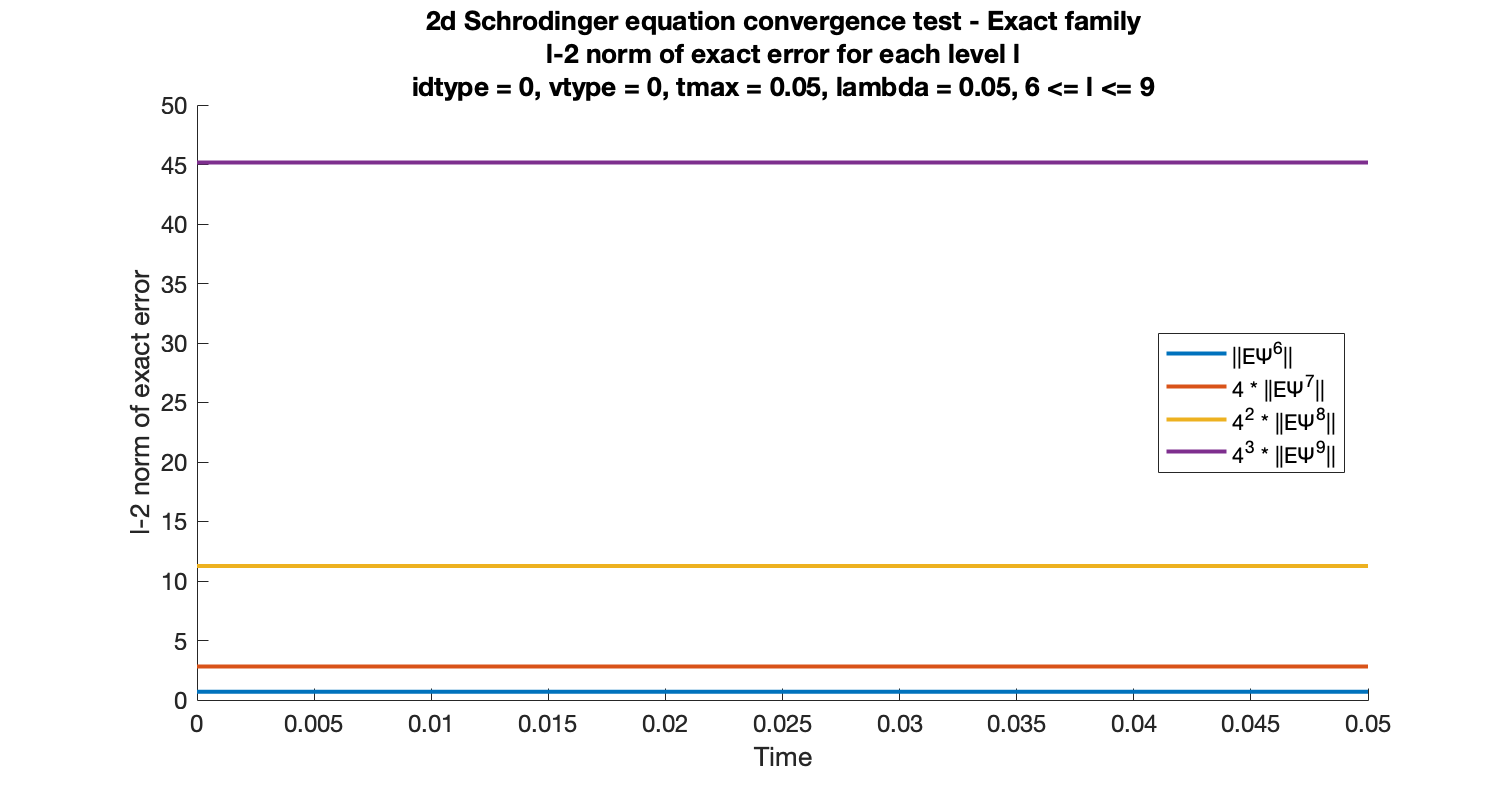
\includegraphics[width=0.95\textwidth]{problem2/ctest_2d-2.png}
\caption{Output 2 of \code{ctest\_2d.m} - 
l-2 norm of exact error at each discretization level.}
\end{figure}

% Describe numerical experiments, show a screenshot from each (double slit show interference)

\begin{figure}[H]
\centering
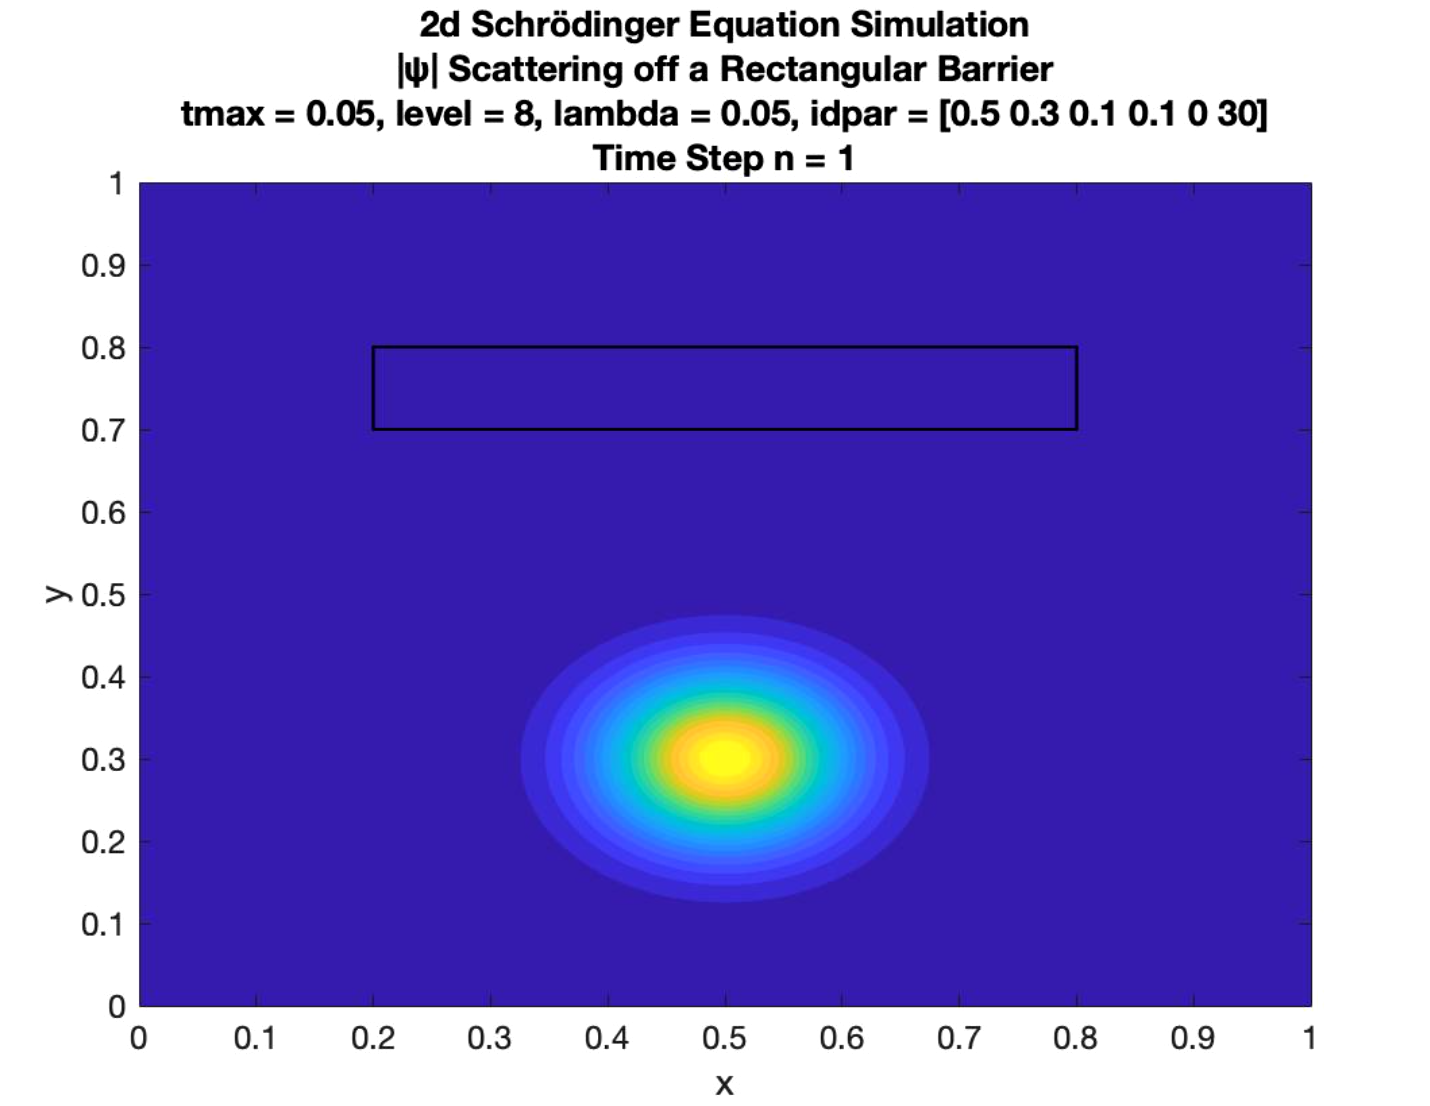
\includegraphics[width=0.75\textwidth]{problem2/rec_bar_1.png}
\caption{Screenshot of video produced by \code{video\_rec\_bar.m} - Initial conditions.}
\end{figure}

\begin{figure}[H]
\centering
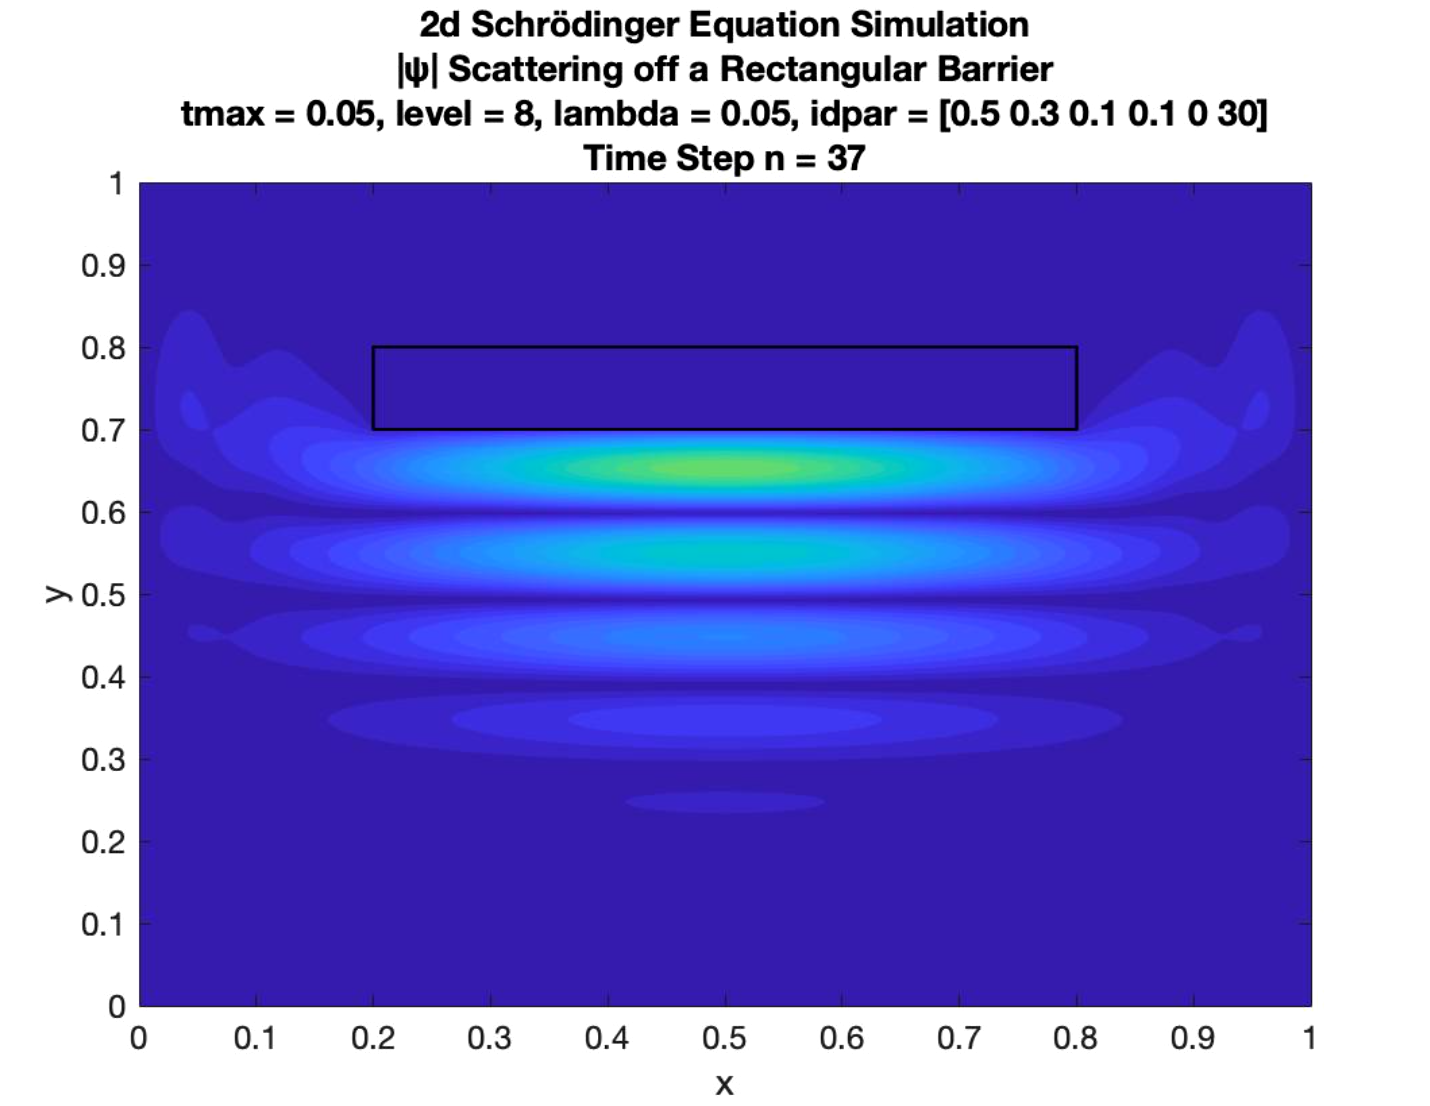
\includegraphics[width=0.75\textwidth]{problem2/rec_bar_2.png}
\caption{Screenshot of video produced by \code{video\_rec\_bar.m} - Scattering off barrier.}
\end{figure}

\begin{figure}[H]
\centering
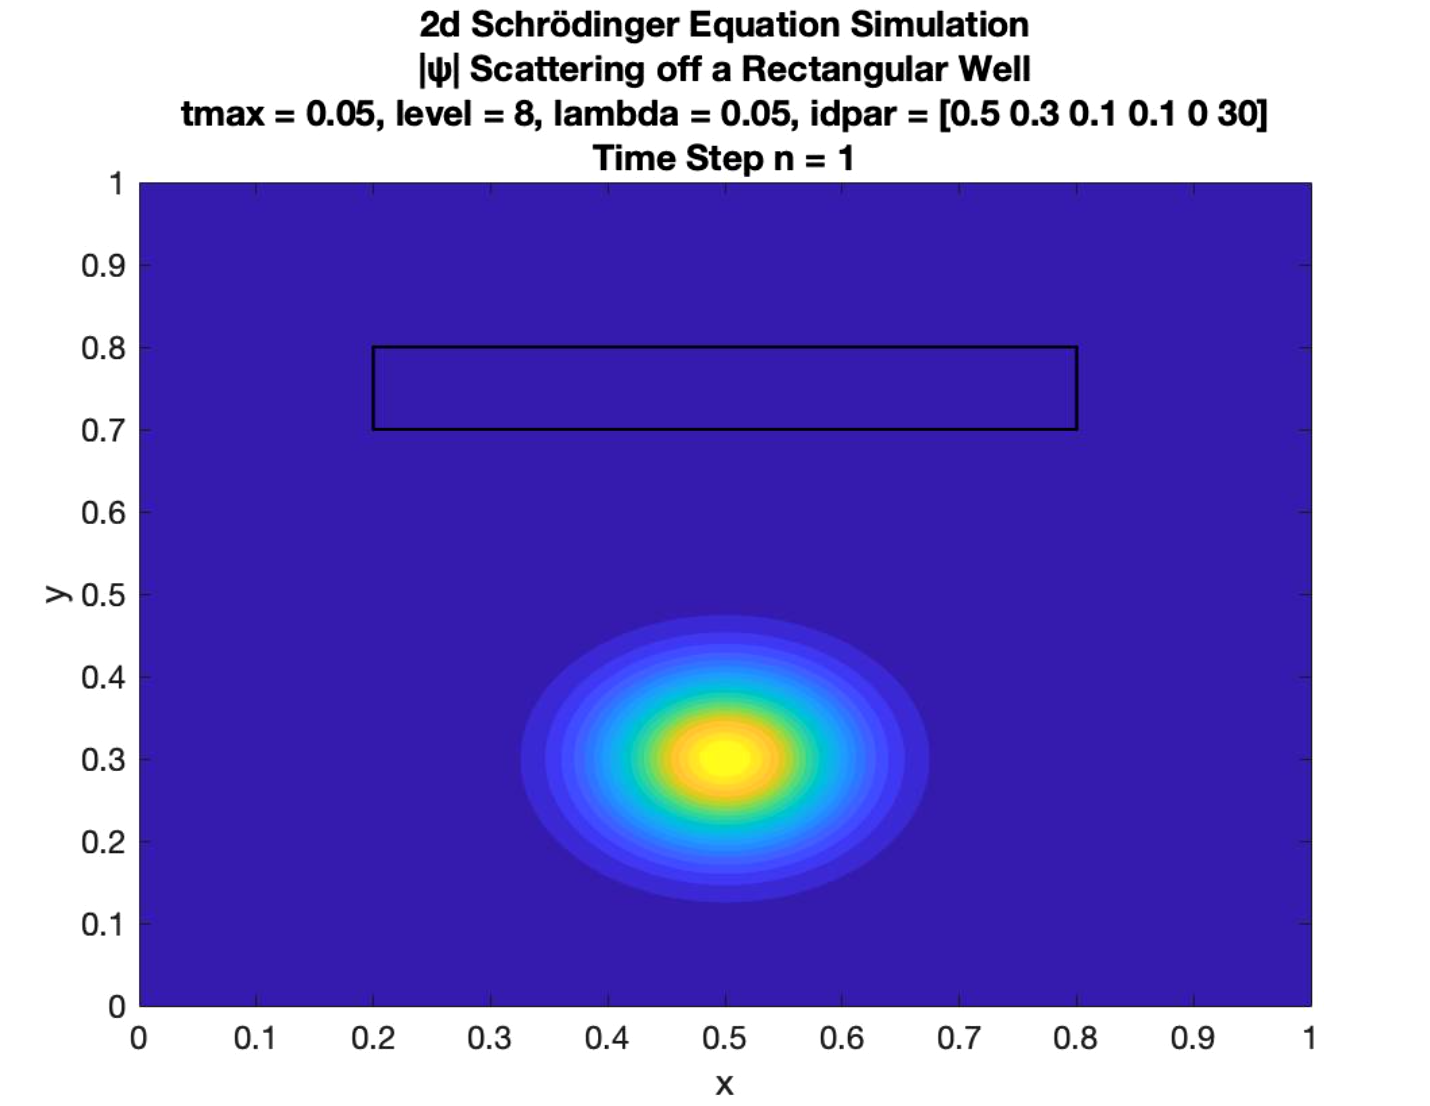
\includegraphics[width=0.75\textwidth]{problem2/rec_well_1.png}
\caption{Screenshot of video produced by \code{video\_rec\_well.m} - Initial conditions.}
\end{figure}

\begin{figure}[H]
\centering
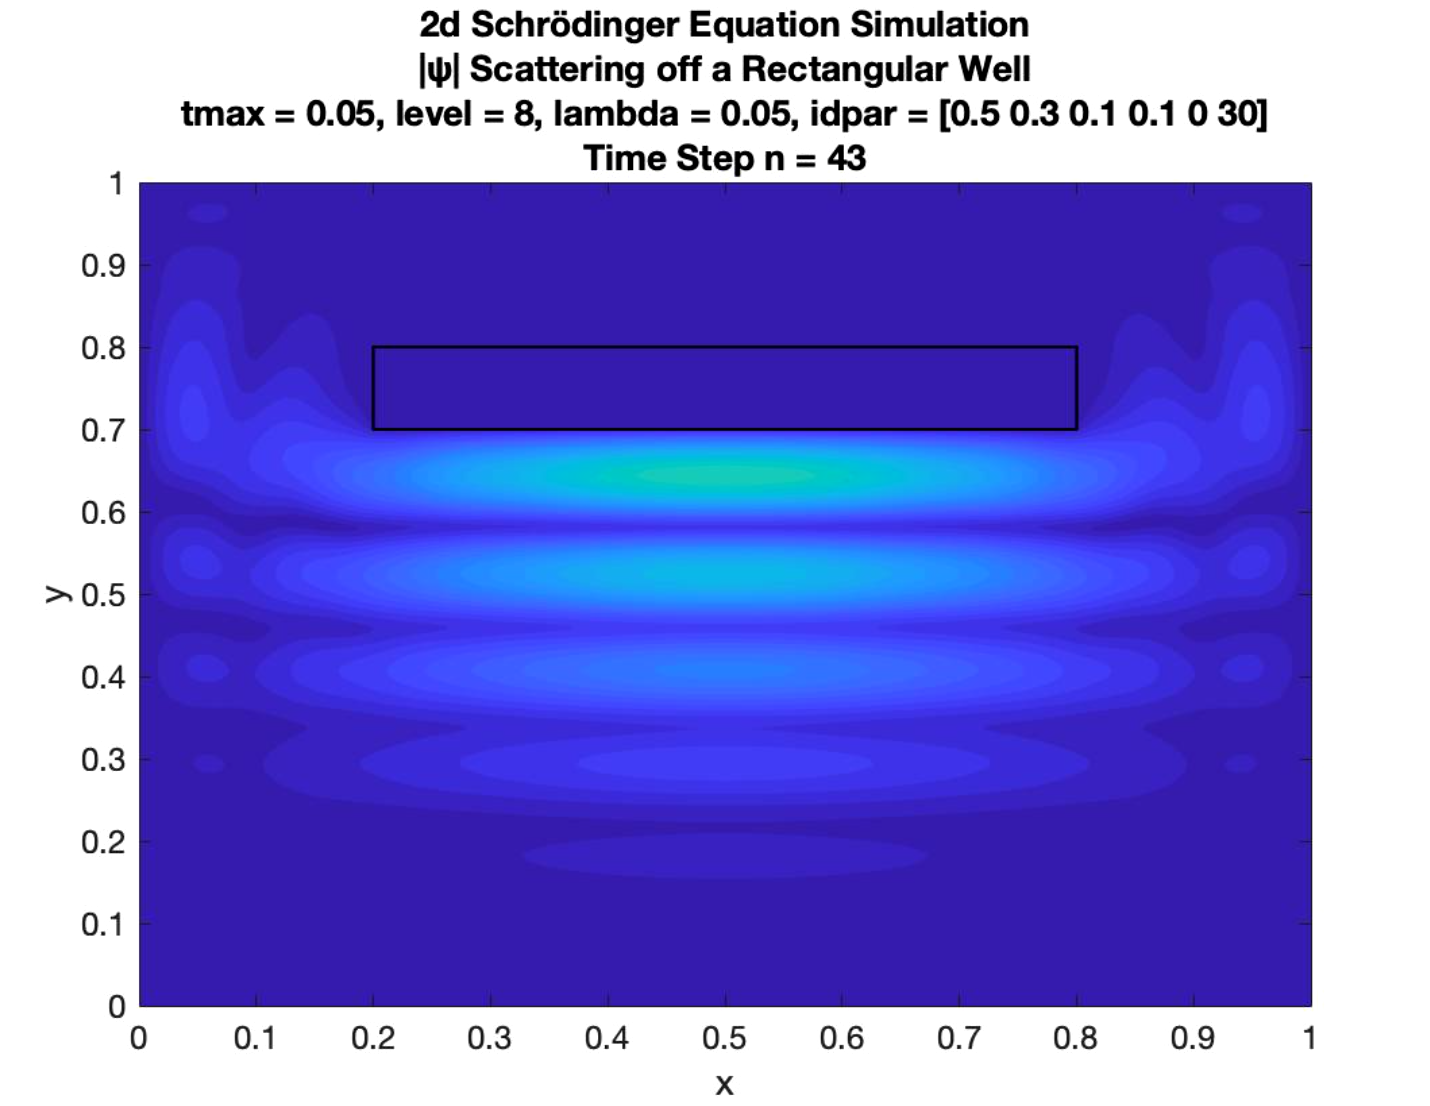
\includegraphics[width=0.75\textwidth]{problem2/rec_well_2.png}
\caption{Screenshot of video produced by \code{video\_rec\_well.m} - Scattering off well.}
\end{figure}

\begin{figure}[H]
\centering
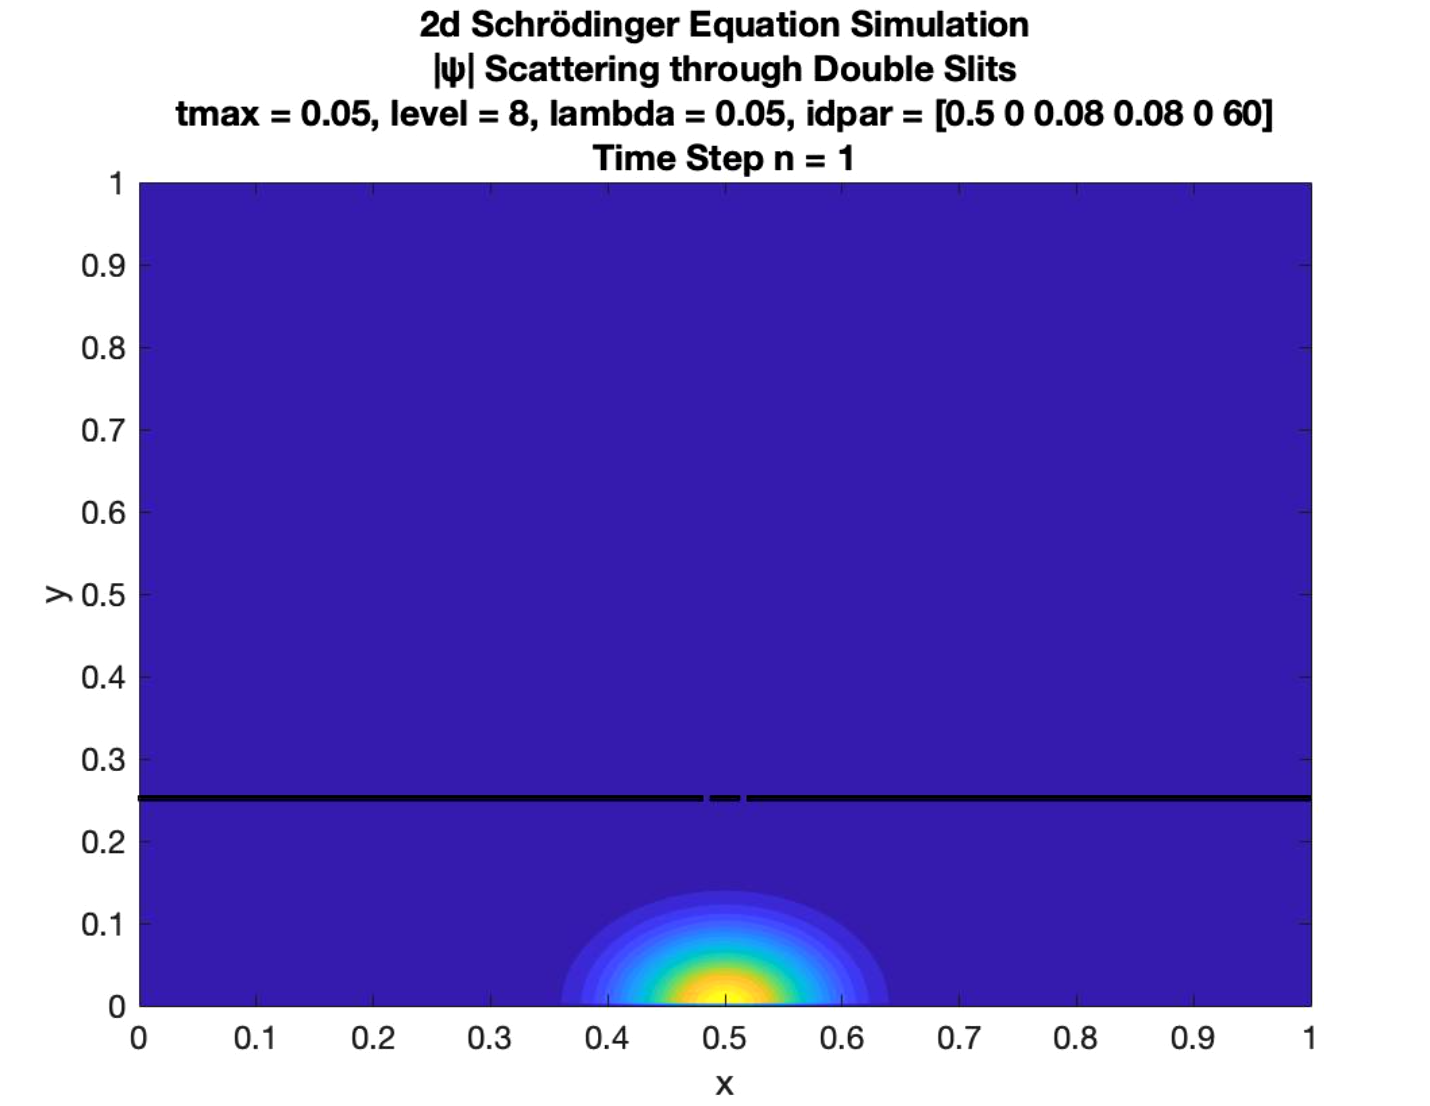
\includegraphics[width=0.75\textwidth]{problem2/double_slit_1.png}
\caption{Screenshot of video produced by \code{double\_slit\_well.m} - Initial conditions.}
\end{figure}

\begin{figure}[H]
\centering
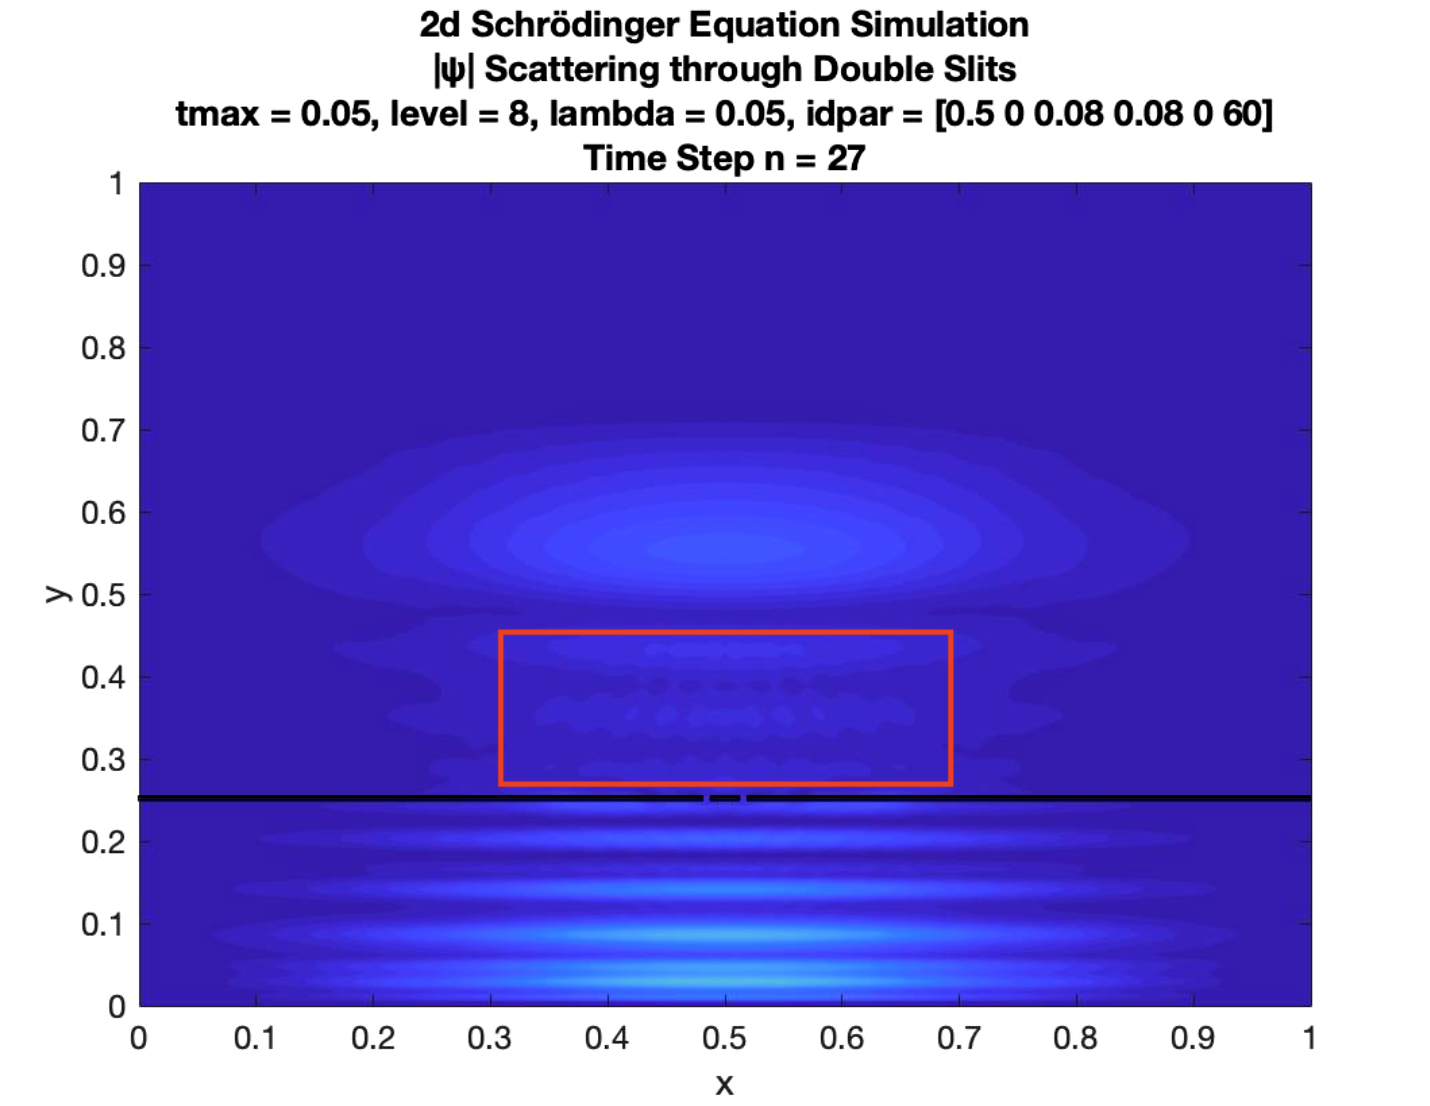
\includegraphics[width=0.75\textwidth]{problem2/double_slit_2.png}
\caption{Screenshot of video produced by \code{double\_slit\_well.m} - 
Self interference through slits.}
\end{figure}


%%%%%%%%%%%%%%%%%%%%%%%%%%%%%%%%%%%%%%%%%%%%%%%%%%%%%%%%%%%%%%%%%%%%%%%%%%%%%%%%%%%%%%%%%%%%%%%%%%%%%%%
% Conclusions
%%%%%%%%%%%%%%%%%%%%%%%%%%%%%%%%%%%%%%%%%%%%%%%%%%%%%%%%%%%%%%%%%%%%%%%%%%%%%%%%%%%%%%%%%%%%%%%%%%%%%%%
\subsection*{Conclusions}

% Summarize work 
% Discuss how mostly successful except for perhaps well survey.

% Talk about performance issues. Could fix by preallocatting memory and using parallel computation.

Generative AI was used to help with understanding how to use MATLAB's \code{contourf} function for 
making videos of numerical experiments in 2d. It was also used for help with typesetting this 
document.

\pagebreak

%%%%%%%%%%%%%%%%%%%%%%%%%%%%%%%%%%%%%%%%%%%%%%%%%%%%%%%%%%%%%%%%%%%%%%%%%%%%%%%%%%%%%%%%%%%%%%%%%%%%%%%
% Appendices
%%%%%%%%%%%%%%%%%%%%%%%%%%%%%%%%%%%%%%%%%%%%%%%%%%%%%%%%%%%%%%%%%%%%%%%%%%%%%%%%%%%%%%%%%%%%%%%%%%%%%%%

\subsection*{Appendix A - sch\_1d\_cn.m Code}
\lstinputlisting{../src/problem1/sch_1d_cn.m}
\pagebreak

\subsection*{Appendix B - ctest\_1d.m Code}
\lstinputlisting{../src/problem1/ctest_1d.m}
\pagebreak

\subsection*{Appendix C - barrier\_survey.m Code}
\lstinputlisting{../src/problem1/barrier_survey.m}
\pagebreak

\subsection*{Appendix D - well\_survey.m Code}
\lstinputlisting{../src/problem1/well_survey.m}
\pagebreak

\subsection*{Appendix E - sch\_2d\_adi.m Code}
\lstinputlisting{../src/problem2/sch_2d_adi.m}
\pagebreak

\subsection*{Appendix F - ctest\_2d.m Code}
\lstinputlisting{../src/problem2/ctest_2d.m}
\pagebreak

\subsection*{Appendix G - video\_rec\_bar.m Code}
\lstinputlisting{../src/problem2/video_rec_bar.m}
\pagebreak

\subsection*{Appendix H - video\_rec\_well.m Code}
\lstinputlisting{../src/problem2/video_rec_well.m}
\pagebreak

\subsection*{Appendix I - video\_double\_slit.m Code}
\lstinputlisting{../src/problem2/video_double_slit.m}
\pagebreak

\end{document}